查看本节演示代码：\demonotebook{05}{5.5_symmetry_enhanced_VQE} \ \demonotebookgithub{05}{5.5_symmetry_enhanced_VQE}

\subsubsection{背景}
变分量子算法主要聚焦于识别复杂多体系统的基态。在这一背景下，变分量子本征求解器（VQE）算法作为一种通过最小化平均能量来寻找多体系统基态的方法，已经成为强大工具。然而，物理中的若干关键现象（包括拓扑相）不仅需要了解基态，还需要了解多个低能本征态。因此，将 VQE 扩展到更高能量本征态具有重要意义。

加权 SSVQE 方法提供了另一种方案，用于生成给定哈密顿量 $H$ 的全部 $k$ 个最低能量本征态~\cite{nakanishi2019subspace}。该方法使用一组 $k$ 个正交初态，记为 $\{|\phi_{i}\rangle\}_{i=1}^{k}$（其中 $\langle \phi_{i} | \phi_{j} \rangle = \delta_{ij}$），作为单个参数化量子线路的输入，该线路由酉算符 $U(\vec{\theta})$ 描述。由于初态彼此正交，由同一线路生成的输出 $U(\vec{\theta})| \phi_{j} \rangle$ 也保持正交。在加权 SSVQE 中，目标是最小化代价函数
\begin{equation}
    \mathrm{cost} = \sum_{i=1}^{k} w_{i} \langle \phi_{i}| U^{\dagger}(\vec{\theta}) H U(\vec{\theta}) | \phi_{i} \rangle,
    \label{ssvqe_cost}
\end{equation}
其中 $w_1 > w_2 > \cdots > w_k$ 为正实数。最小化式~\eqref{ssvqe_cost} 中的代价函数会产生全部 $k$ 个最低能量本征态，使得 $|E_{i}\rangle = U(\vec{\theta}^{*})|\phi_{i}\rangle$。
加权 SSVQE 的一个显著优势是，它可以通过一次优化过程给出全部 $k$ 个最低能量本征态，而不需要评估量子态重叠。然而，随着目标本征态数量增加，该算法对资源的需求也会提高。

对称性是物理学，尤其是量子力学中最基本的概念之一。多数物理系统都表现出各种类型的对称性，并可通过数学方式准确描述。将这些对称性纳入 VQE 算法也能显著提升算法表现。将对称性引入 VQE 算法有两种方式：（i）设计能够自然生成具有相关对称性的量子态的线路~\cite{Lyu2020accelerated,Gard2020,barron2021preserving}；（ii）在代价函数中添加额外项，用于惩罚不具备相关对称性的量子态~\cite{mcclean2016theory,ryabinkin2018constrained}。

\subsubsection{实现}
利用 \MindQuantum\ 灵活且全面的功能，研究人员可以通过定义自定义目标函数来处理多种优化目标。本节演示如何使用 \MindQuantum\ 实现 SSVQE，并结合多种对称性策略，精确确定 Heisenberg 哈密顿量的四个最低态能量。

首先，需要构造保持对称性的 ansatz，详细内容见文献~\cite{Lyu2023symmetryenhanced}。
\begin{lstlisting}
def entangling_gate(parameter, qubits):
    circuit = Circuit()
    circuit += RZ(-np.pi / 2).on(qubits[1])
    circuit += CNOT.on(qubits[0], qubits[1])
    circuit += RZ({parameter: -2}).on(qubits[0])
    circuit += RZ(np.pi / 2).on(qubits[0])
    circuit += RY({parameter: 2}).on(qubits[1])
    circuit += RY(-np.pi / 2).on(qubits[1])
    circuit += CNOT.on(qubits[1], qubits[0])
    circuit += RY({parameter: -2}).on(qubits[1])
    circuit += RY(np.pi / 2).on(qubits[1])
    circuit += CNOT.on(qubits[0], qubits[1])
    circuit += RZ(np.pi / 2).on(qubits[0])
    return circuit

def ansatz(N, layers, local_rot=True):
    circuit = Circuit()
    params_index = 0
    for layer_index in range(layers):
        for i in range(2):
            for j in range(i, N - 1, 2):
                circuit += entangling_gate(str(params_index), [j, j + 1])
                params_index += 1
        if local_rot:
            for i in range(N):
                circuit += PhaseShift(params_index).on(i)
                params_index += 1
    return circuit
\end{lstlisting}

SSVQE 可以实现为多个 VQE 的组合，每个 VQE 具有不同初始化线路，但共享同一个参数化 ansatz。
对于多数 VQE 实例，具体任务由其对应测量函数定义。
使用 \getexpectationwithgrad\ 函数，可以方便地获得期望值及其关于可训练变量的对应梯度。这里以 Heisenberg 哈密顿量的第二和第三低能态能量为例，展示代码实现。在该具体实例中，
我们使用一个保持 $S_z$ 守恒的 ansatz，它保持总自旋的 $z$ 分量，并将总自旋算符作为惩罚项加入代价函数。代价函数随后修改为如下形式：
\begin{equation}
    \mathrm{cost} = \sum_{i=1}^{k} w_{i} \langle \phi_{i}| U^{\dagger}(\vec{\theta}) [H + \beta(\hat{O} - c)^2] U(\vec{\theta}) | \phi_{i} \rangle,
    \label{ssvqe_cost_pen}
\end{equation}
其中 $c$ 是表示目标子空间的常数，$\beta$ 是正的常数，其取值会根据惩罚项形式设置得足够大。这里展开 $(\hat{O} - c)^2 {=} \hat{O}^2 {-} c\hat{O} {+} c^2$。连同哈密顿量在内，我们现在有三个不同测量算符。Heisenberg 哈密顿量和总自旋算符情形下的相应测量算符可以通过以下代码生成。

\begin{lstlisting}
def s_alpha(N, alpha: str = 'X'):
    alpha = alpha.upper()
    out = QubitOperator()
    for i in range(N):
        out += QubitOperator(alpha + f'{i}')
    return out * 0.5

def s_tot_op(N):
    s_x_op = s_alpha(N, 'X')**2
    s_y_op = s_alpha(N, 'Y')**2
    s_z_op = s_alpha(N, 'Z')**2
    op = s_x_op + s_y_op + s_z_op
    op.compress()
    return op

def ham_heis(n_qubits, J):
    ham = QubitOperator()
    for i in range(1, n_qubits):
        ham += QubitOperator("X{} X{}".format(i - 1, i), J)
        ham += QubitOperator("Y{} Y{}".format(i - 1, i), J)
        ham += QubitOperator("Z{} Z{}".format(i - 1, i), J)
    ham.compress()
    return Hamiltonian(ham)
\end{lstlisting}

预先定义初始化线路、共享参数 ansatz、测量算符和常数 $\beta$ 等所有必要模块后，就可以继续实现 SSVQE 算法。以下代码片段展示了 SSVQE 类的实现。
\begin{lstlisting}
class SSVQE:
    def __init__(self, n_qubits, init_circuits, pqc, ops, beta):
        self.n_qubits = n_qubits
        self.circs = [circ + pqc for circ in init_circuits]
        self.sim = Simulator('mqvector', n_qubits)
        self.beta = beta
        self.grad_ops = [self.sim.get_expectation_with_grad(ops, circ) for circ in self.circs]

    def energy(self, params):
        if self.sim is None:
            self.sim = Simulator('mqvector', self.n_qubits)
        energies = []
        for i in range(len(self.grad_ops)):
            f, g = self.grad_ops[i](params)
            energies.append(f[0, 0].real)
        return energies

    def __call__(self, inputs):
        cost = 0
        cost_grad = 0
        for i in range(len(self.grad_ops)):
            f, g = self.grad_ops[i](inputs)
            f1, f2, f3 = f[0, 0].real, f[0, 1].real, f[0, 2].real
            g1, g2, g3 = np.array(g[0, 0, :].real), np.array(g[0, 1, :].real), np.array(g[0, 2, :].real)
            cost += (f1 + self.beta * (f2 + f3)) * (len(self.grad_ops) - i)
            cost_grad += (g1 + self.beta * (g2 + g3)) * (len(self.grad_ops) - i)
        return cost, cost_grad
\end{lstlisting}


完成算法实现后，重点转向 SSVQE 优化。经典优化器的选择仍然是灵活的。在本例中，选择 SciPy 中的 \code{"L-BFGS-B"} 优化器。


\begin{lstlisting}
initial_parameter = (np.random.rand(len(ssvqe.circs[0].params_name)) - .5) * np.pi
res = scipy.optimize.minimize(ssvqe,
                    initial_parameter,
                    method='l-bfgs-b',
                    jac=True,
                    options={'disp': False})
\end{lstlisting}

\begin{figure}
	\centering
	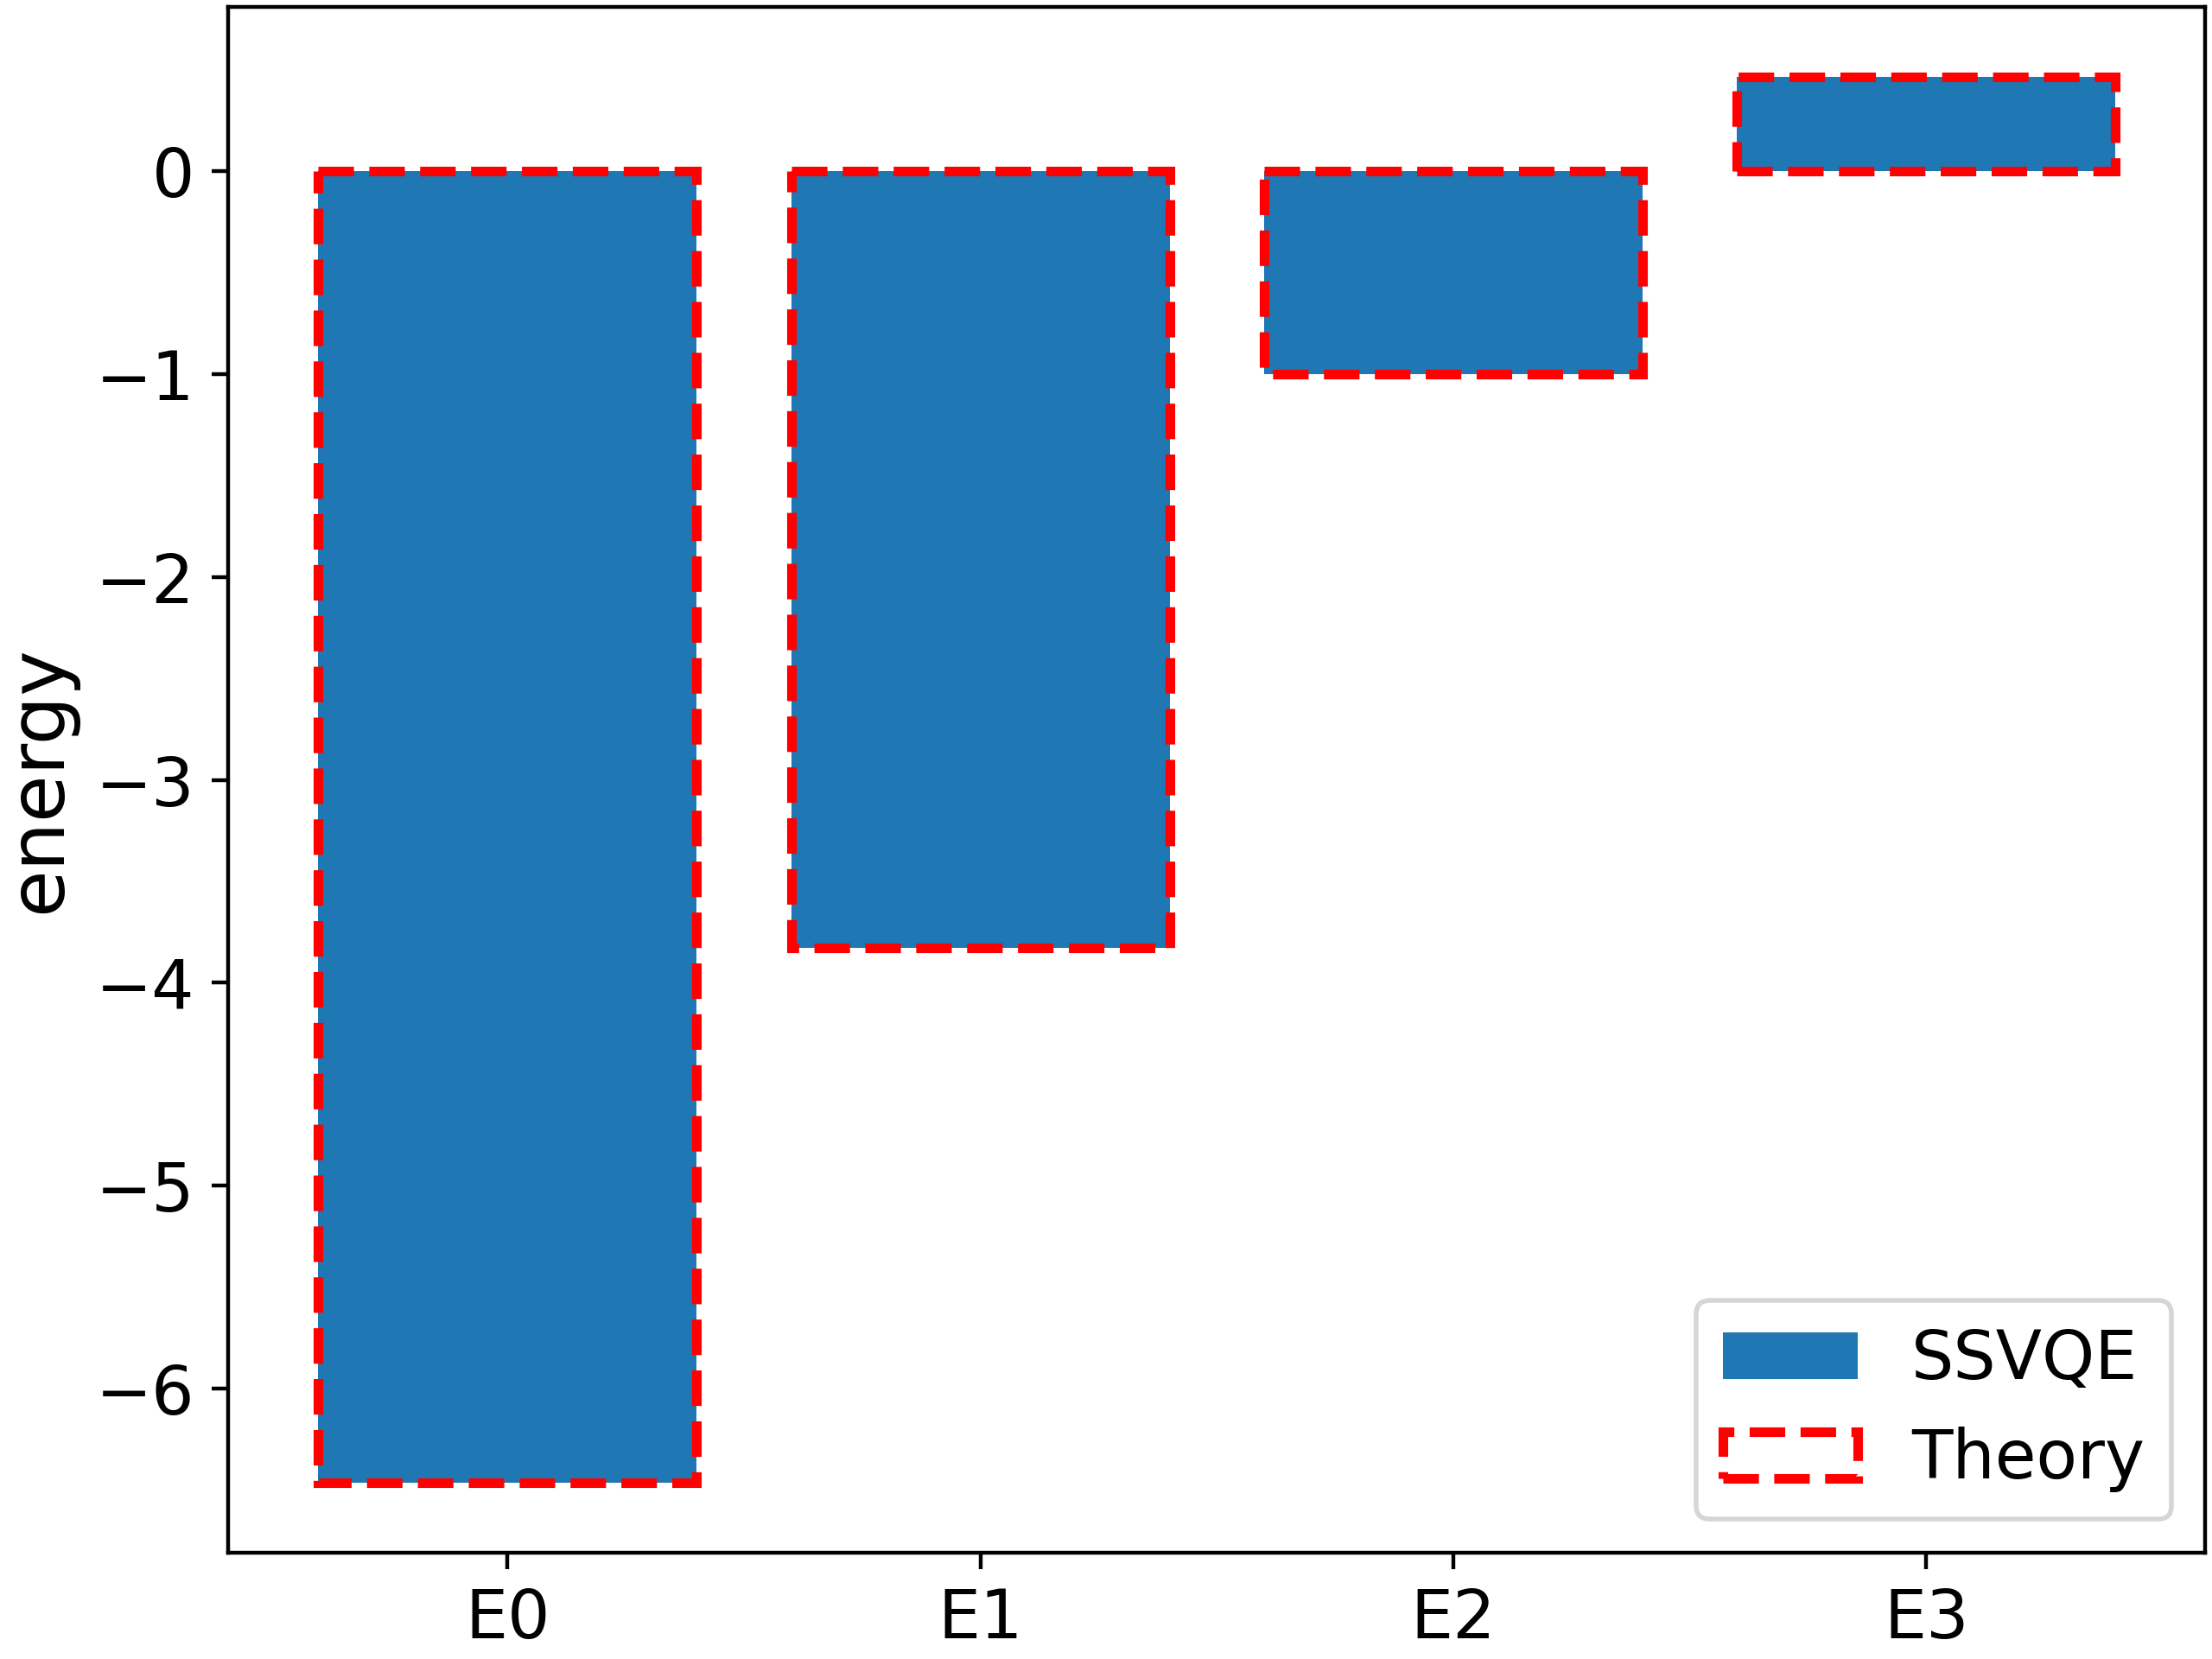
\includegraphics[width=1\linewidth]{5.4.2_figure/result.png}
	\caption{结合对称性的 SSVQE 在 4 量子比特 Heisenberg 哈密顿量上的模拟结果}
	\label{fig:SSVQE_result}
\end{figure}

该实现只需数秒即可完成 4 量子比特 Heisenberg 哈密顿量的训练。可以查看最终结果，并生成图像比较近似结果与理论能量。图~\ref{fig:SSVQE_result} 展示了 $4$ 量子比特 Heisenberg 哈密顿量四个最低态能量的模拟结果。显然，通过在 SSVQE 中纳入内在对称性，可以以资源高效的方式精确近似基态和激发态能量。
